\section{Ajout du Bruit Blanc Gaussien }
Le bruit blanc gaussien est un type de bruit aléatoire dont les échantillons sont tirés d'une distribution gaussienne c'est à dire, un bruit aléatoire dont les composantes réelles et imaginaires suivent une distribution normale. Ici, une moyenne nulle et un écart type de 1 ont été considérés.
Dans le code python celui ci est ajouté via la fonction \texttt{add\_awgn}.

En calculant le Rapport Signal sur Bruit (SNR) pour différentes valeurs, une atténuation des amplitudes des signaux reçus avec bruit devient visible, due au fait que la puissance du bruit ajouté rend plus difficile la distinction entre le bruit et le signal. Un faible SNR engendre une grande puissance de bruit (\ref{eq:p_bruit}), compliquant ainsi la distinction entre signal et bruit. De plus, l'ajout d'un SNR négatif conduit à un \textit{SNR\_linear} < 1, ce qui signifie que $P_{\text{bruit}} > P_{\text{signal}}$. Le radar FMCW détecte alors des cibles fantômes et atténue l'amplitude des signaux réels. Ceci s'illustre bien sur la comparaison des RDM qui est faite sur la figure \ref{fig:rdm_wn} pour différents valeurs de SNR.

\begin{figure}[H]
    \centering
    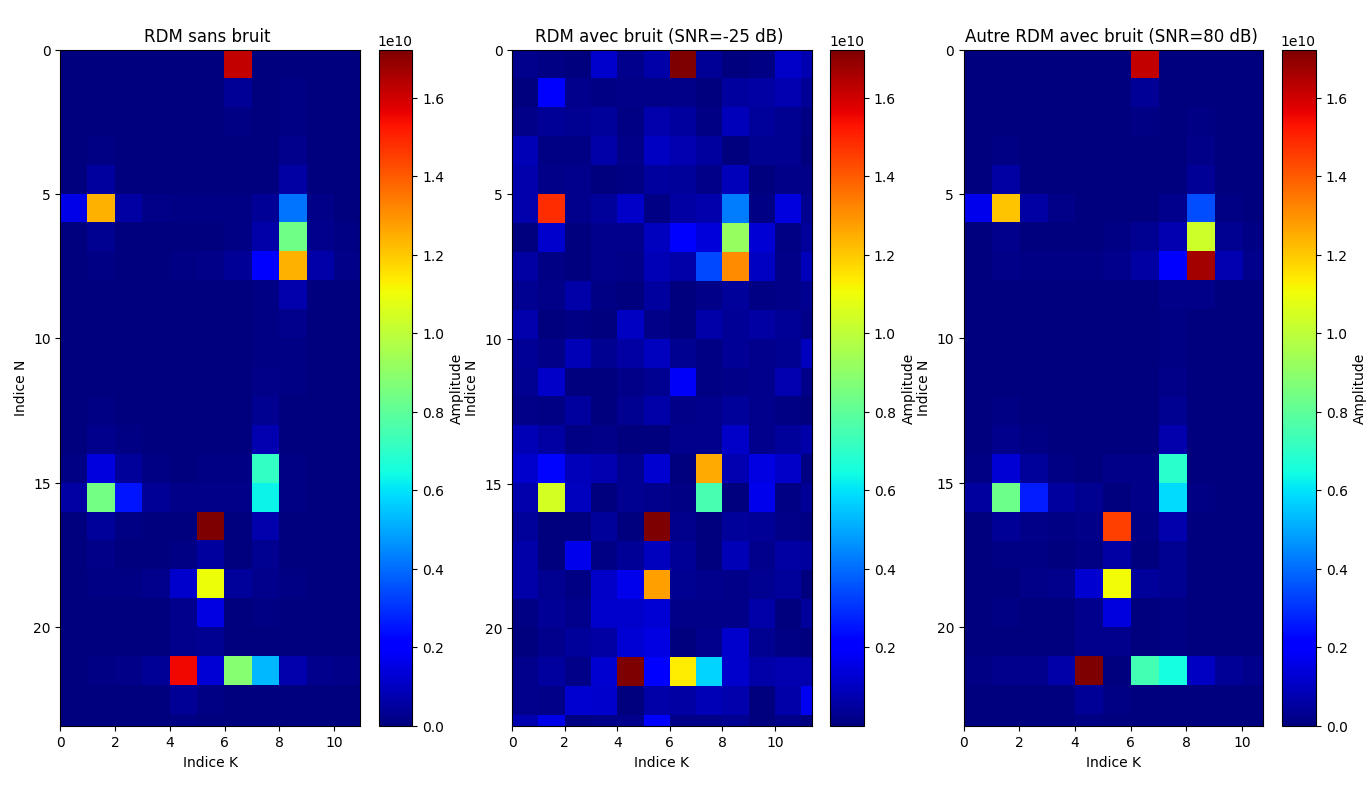
\includegraphics[width=0.77\textwidth]{Pictures/RDM_WITH_WITHOUT_SST_P.png}
    \caption{Comparaison entre RDM avec et sans bruit pour différentes valeurs de SNR}
    \label{fig:rdm_wn}
\end{figure}